\documentclass[
11pt,%
tightenlines,%
twoside,%
onecolumn,%
nofloats,%
nobibnotes,%
nofootinbib,%
superscriptaddress,%
noshowpacs,%
centertags]%
{revtex4}
\usepackage{ljm}
\usepackage{listings}

\lstset{
language=C++,
basewidth=0.5em,
xleftmargin=45pt,
xrightmargin=45pt,
basicstyle=\small\ttfamily,
keywordstyle=\bfseries\underbar,
numbers=left,
numberstyle=\tiny,
stepnumber=1,
numbersep=10pt,
showspaces=false,
showstringspaces=false,
showtabs=false,
frame=trBL,
tabsize=2,
captionpos=t,
breaklines=true,
breakatwhitespace=false,
escapeinside={\%*}{*)}
}

\begin{document}

\titlerunning{dataflow processor emulator}
\authorrunning{Shabanov et al.}

\title{Features of Dataflow Processor Emulator Implementing}

\author{\firstname{B.~M.}~\surname{Shabanov}}
\email[E-mail: ]{shabanov@jscc.com}
\affiliation{Joint Supercomputer Center of the Russian Academy of Sciences -- branch of Scientific Research Institute of System Analysis of the Russian Academy of Sciences, Leninsky prospect 32a, Moscow, 119334, Russia}

\author{\firstname{E.~A.}~\surname{Kuznetsova}}
\email[E-mail: ]{mrallis@jscc.com}
\affiliation{Joint Supercomputer Center of the Russian Academy of Sciences -- branch of Scientific Research Institute of System Analysis of the Russian Academy of Sciences, Leninsky prospect 32a, Moscow, 119334, Russia}

\author{\firstname{A.~A.}~\surname{Rybakov}}
\email[E-mail: ]{rybakov.aax@gmail.com}
\affiliation{Joint Supercomputer Center of the Russian Academy of Sciences -- branch of Scientific Research Institute of System Analysis of the Russian Academy of Sciences, Leninsky prospect 32a, Moscow, 119334, Russia}

\author{\firstname{S.~S.}~\surname{Shumilin}}
\email[E-mail: ]{shumilin@jscc.com}
\affiliation{Joint Supercomputer Center of the Russian Academy of Sciences -- branch of Scientific Research Institute of System Analysis of the Russian Academy of Sciences, Leninsky prospect 32a, Moscow, 119334, Russia}

\firstcollaboration{(Submitted by S.~S.~Submitter)}

\received{May 01, 2020}

\begin{abstract}
The development of dataflow processor architecture is a promising direction for improving the performance of computing systems.
The dataflow processors has several advantages in contrast with processor with the von Neumann architecture. 
These advantages are express in explicit parallelism of calculations, since in the presentation of programs for the dataflow processor the sequence of instructions limited solely by the fact of input data’s ready state.
The concept of using tokens as data storage for instructions allows you to remove many problems associated with data conflicts and simplifies the program logic.
One of the most important elements in the implementation of the logic of the dataflow processor is the content-addressable token memory, which should provide storage and quick search for ready-made data for instructions that can be transfer for execution.
This article discusses the functionality of the dataflow processor emulator and its parts including content-addressable token memory and the logic of its operation using the example of a simple dataflow graph.
\end{abstract}

\subclass{68N20,68R10} % Enter 2010 Mathematics Subject Classification.

\keywords{Dataflow processor emulator, dataflow graph, token, token state, associative memory, control flow graph, def-use graph.}

\maketitle

\section{Introduction}

The processor with dataflow architecture (the dataflow processor) has the potential to provide the highest performance among processors due the fact that parallelism of programs execution laying down since program graph created.
Thereby performance is not required to be detected using sophisticated equipment from the sequence of instructions specified by the instruction counter, as is the case in a processor with the von Neumann architecture.
A program in the dataflow processor is the oriental graph where nodes are instructions and information transfers by the arcs as tokens, which contains the data field and context field of transferring data.
This context absolutely identifies where token should transfers (the number of receiver command in the graph) and also contains the number of index, iteration and the subprogram execution, which allow to execute different iterations of inner cycles and different executions of procedures at the same program graph at parallel.
Regardless of the place of the two-input instruction in the graph, it transfers for execution upon arrival at the input of the last of the pair of operand tokens with the same context.
After the execution the result in the actuator, new tokens with the result value sends to the inputs of subsequent commands according to the program column, and the used operands destroys.

At the same time, in contrast to the von Neumann architecture, the dataflow processor has not a central control device (instruction counter), and the parallelism of the executing instructions determined in dynamics by the arrival of operands to the instruction inputs in the decentralized scheme.
Namely, the device for searching ready-to-execute commands -- the memory of searching pairs (the content-addressable memory) can be executed such as many parallel-running modules, which provides the same large numbers of actuators \cite{fine-grained-prl}.

In contrast with the well-known projects of vector dataflow machines, in which arithmetic operations on vectors performs only for vectors in their registers, the block of vector register is absent in the dataflow processor emulator and a single-level memory of high-capacity vectors (RAM level) is using.
This eliminates the problem of the possibility of overflow on the register file, which does not have a simple solution, given the complete asynchrony of the dataflow model of calculating.
Besides it is necessary to execute 2-3 times more commands in dataflow processor on scientific tasks compared to the von Neumann processor \cite{multithreading}.
It is also not so easy to do without the participation of the operating system in the process of the program execution when allocating space for the created arrays in the main memory.
Therefore, it proposed to implement the distribution of the vector memory resource in the dataflow processor emulator at the hardware level \cite{vpp}.

The difficulties noted above for the hardware implementation of the dataflow processor led to the fact that none of the many projects for its creation was not possible to achieve higher performance compared to the von Neumann processor, and by the end of the 2000s, there were practically no such projects.
This refers to the development of universal dataflow processors, but not specialized ones, since, for example, dataflow processors of digital signal processing were not only developed, but also produced \cite{terada}.

Unlike the implementation on a multiprocessor system, direct hardware implementation allows you to fully implement the calculation graph in the form of a computing pipeline, thereby eliminating the need to create a module that implements the execution of the calculation schedule \cite{popov}.

\section{Processor with The von Neumann architecture emulation}

One of the basic principles of the von Neumann architecture is the principle of program control sequence.
According to it, the executable code of the program is stored in memory, and the processor can execute its instructions sequentially, one by one.
The next instruction address submitted to the processor for execution is stored in a special register called instruction pointer.
By default, it always shifts to the next instruction in memory.
This address can be forcedly changed by special transition instructions, and in this case we can talk about transferring control to another part of the program.

We introduce the concept of a linear section (or the program base block).
The linear section is a sequence on instructions with the next two properties.
Firstly, control could only be transfer to the first instruction of a given section.
In other words, a linear section has only one input, which is the first section instruction.
Secondly, if control was transfer to the linear section than all instructions of this section must be done (i.e., there can be no transition instructions inside the linear section).
The transition instruction can only be at the end of the linear section.
Sometimes, instead of linear sections, it is convenient to view so-called quasilinear sections, which can have arbitrary amount of transition instructions inside for transitions to other linear sections.
We will not review quasilinear sections, because any such section can be split into a sequence of ordinary linear sections.

An important concept widely used in the theory of optimizing compilers is the control flow graph (CFG) \cite{Muchnick}.
A control flow graph is a directed graph whose nodes are linear sections of the program, and arcs indicate the transfer of control between them.
The control flow graph is a convenient and visual structure for describing program behavior and used by optimizing compilers to implement global program optimizations i.e. optimizations that go beyond linear sections.

Consider the logic of the device intermediate program representation inside one linear section.
Consider for this a simple example of finding roots of a quadratic equation.
We will use listing in the C programming language to write examples and pseudocode.
So, let us have a linear section (program code block) at the input of which we have the variables $a$, $b$, $c$ containing the coefficients of the quadratic equation $ax^2 + bx + c = 0$.
At the linear section output it is required to get the values of the roots, which are calculated by the formulas $x_{1,2} = (-b \pm \sqrt{b^2 - 4ac})/(2a)$.

\begin{lstlisting}[caption={The code block for calculating the roots of the quadratic equation.},label={lst:square_equation_1}]
{
    float t = sqrt(b * b - 4.0 * a * c);
    
    x1 = (-b + t) / (2.0 * a);
    x2 = (-b - t) / (2.0 * a);
}
\end{lstlisting}

\

In Listing~\ref{lst:square_equation_1}, linear section is delimited in curly brackets and a temporary variable $t$ is declared to understand that this variable is not used outside the linear section.
For convenience, we assume that the processor, for which the executable code will be created, supports the instruction for calculating the square root.
Thus, the following instructions for working with real numbers will figure in the listing above: MUL -- multiplication of two numbers, SUB -- subtraction of two numbers, SQRT -- square root of number, NEG -- unary negative, ADD -- addition of two numbers, DIV -- division of two numbers.

\begin{figure}[h]
\setcaptionmargin{5mm}
%\onelinecaptionsfalse % if the caption is multiline
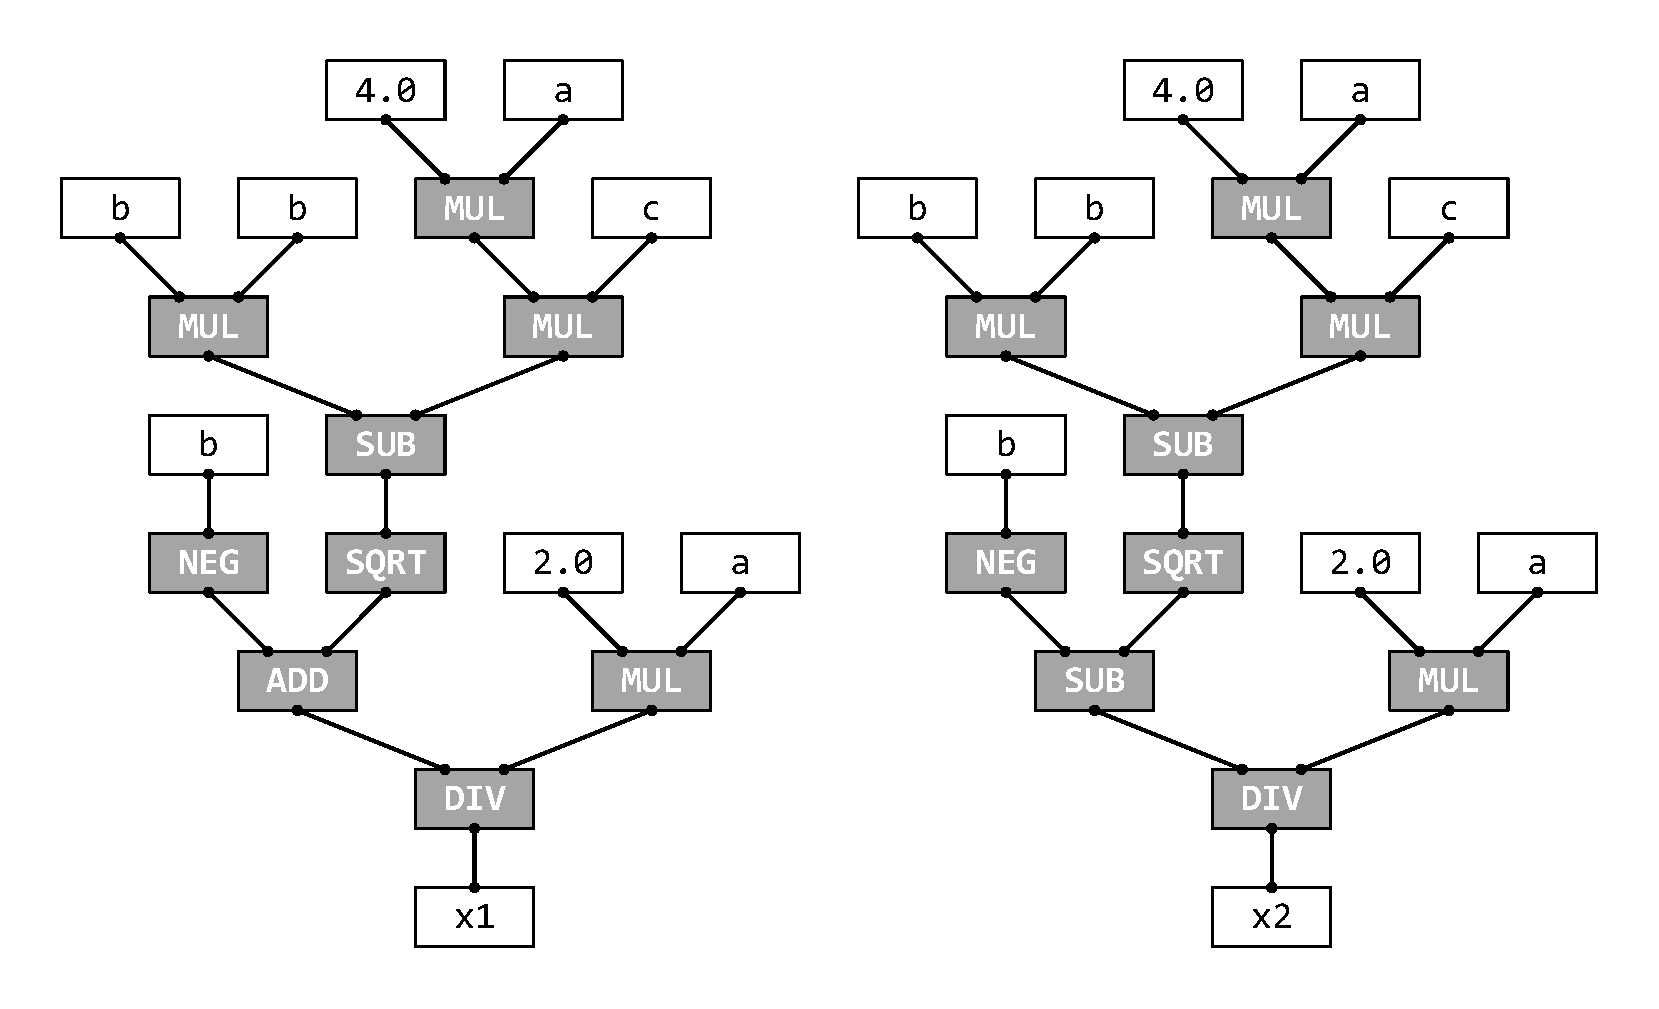
\includegraphics[width=0.95\textwidth]{pics/square_equation_calculation_tree.pdf}
\captionstyle{normal}\caption{Tree for calculating the expressions of the roots of the quadratic equation.}\label{fig:square_equation_calculation_tree}
\end{figure}

Figure~\ref{fig:square_equation_calculation_tree} shows two trees of evaluating the expressions $x_1$ and $x_2$.
The compiler, of course, will simplify the calculation data by collecting common subexpressions, and the final version of the linear section representation will be close to the next dependency graph shown in Figure~\ref{fig:def_use} (def-use graph, DFG).

\begin{figure}[h]
\setcaptionmargin{5mm}
\onelinecaptionsfalse % if the caption is multiline
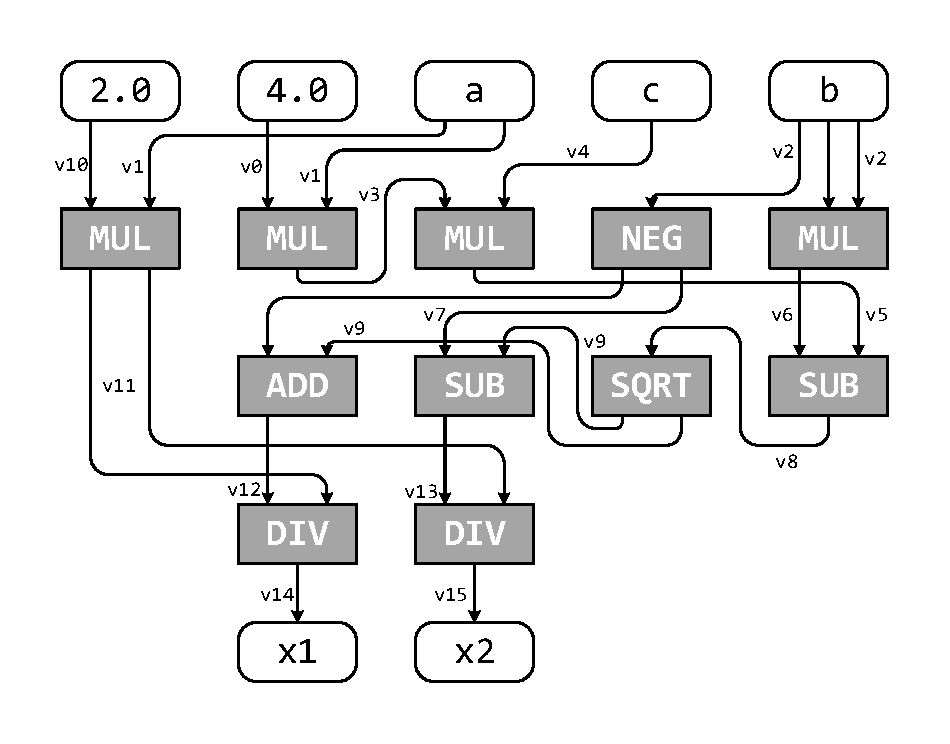
\includegraphics[width=0.60\textwidth]{pics/def_use.pdf}
\captionstyle{normal}\caption{The dependency graph of the linear section in the calculation \\ of the expressions of the roots of the quadratic equation.}\label{fig:def_use}
\end{figure}

Nodes of this directed graph are separate operations (shows dark rectangles), and arcs are use-define chains between data operations (the $B$ command depends on the data from the $A$ command if it consumes the data generated by the $A$ command).
It can be other dependency between operations besides data dependency (control dependency, anti-dependency), but these dependency are missing in our simple example.

To form the resulting executable code the presence of a def-use graph is not enough.
It is necessary to line up all commands included in the def-use graph in a single sequence, which will subsequently be written to a linear section of memory.
In this case, when alignment a sequence of commands, it is necessary to observe the requirement that if the $B$ command depends on the $A$ command according to the data, then it should be later than the $A$ command in the final sequence.
This process called the code planning \cite{Aho}.
In the result of the code planning for considering case we will get pseudocode for calculating the roots of the quadratic equation is such view, shown in Listing~\ref{lst:square_equation_2}.

\begin{lstlisting}[caption={Pseudocode for calculating the roots of a quadratic equation.},label={lst:square_equation_2}]
MOV 4.0       ->  v0
MOV   a       ->  v1
MOV   b       ->  v2
MUL  v0,  v1  ->  v3
MOV   c       ->  v4
MUL  v3,  v4  ->  v5
MUL  v2,  v2  ->  v6
NEG  v2       ->  v7
SUB  v6,  v5  ->  v8
SQRT v8       ->  v9
MOV 2.0       -> v10
MUL v10,  v1  -> v11
ADD  v7,  v9  -> v12
SUB  v7,  v9  -> v13
DIV v12, v11  -> v14
DIV v13, v11  -> v15
MOV v14       ->  x1
MOV v15       ->  x2
\end{lstlisting}

\

In Listing~\ref{lst:square_equation_2}, all instructions except transmission operation operate on virtual registers (v0-v15).
The order of the commands is important in this note.
At any time after the execution of any instruction, we can talk about some state of the processor which characterized by the contents of the memory, as well as all the registers used.

The main part of processor emulator is the realization of instruction semantic, executed by the processor.
I.e. that every instruction is considered as function, which transfers calculating machine from one state to another.

\section{Dataflow processor emulation}

The dataflow processor emulator, which considered in this article, has the dynamic model.
It permits to give away the commands for execution when their tokens are ready with the simultaneous execution possibility of inner cycle’s iterations and different procedure launches on the same program graph.

The dynamic model of the dataflow processor allows revealing more parallelism in the program due to not only the coincidence of the command number of the operand tokens, but also several fields, for example, index number, iteration, and subroutine start \cite{Wiley}.

In contrast with processors with the von Neumann architecture, dataflow processors completely orderliness in command execution.
I.e. if two anyone instructions can execute in parallel (this is possible in the absence of dependence between them) then the order of their execution is not determined.
We will consider the same example of the linear section, inside which the roots of the quadratic equation are calculated.
The program for dataflow processor is the graph just like def-use graph showed at Figure~\ref{fig:def_use}.
Dataflow graph, which is a program for dataflow processor, is also oriented.
Nodes of this graph also are the instructions, but arcs have a completely different meaning.
In the case of def-use graph, arcs were fix fact of the dependence between two operations (indicating by which variables, by which resource), in case of dataflow graph the arc is a unique data carrier that names token.
Therefore, token is a data structure that storage the information about transferring data and about destination point of this data (the identifier consuming this instruction data as well as the argument number, which this data is for the instruction).
Besides, the token contains additional information (the token state) allowing distinguishing instruction, which relate to different function process or to different cycle iteration, but for this example, this is not important, therefore, the description of token state will omitted.

\begin{figure}[h]
\setcaptionmargin{5mm}
\onelinecaptionsfalse % if the caption is multiline
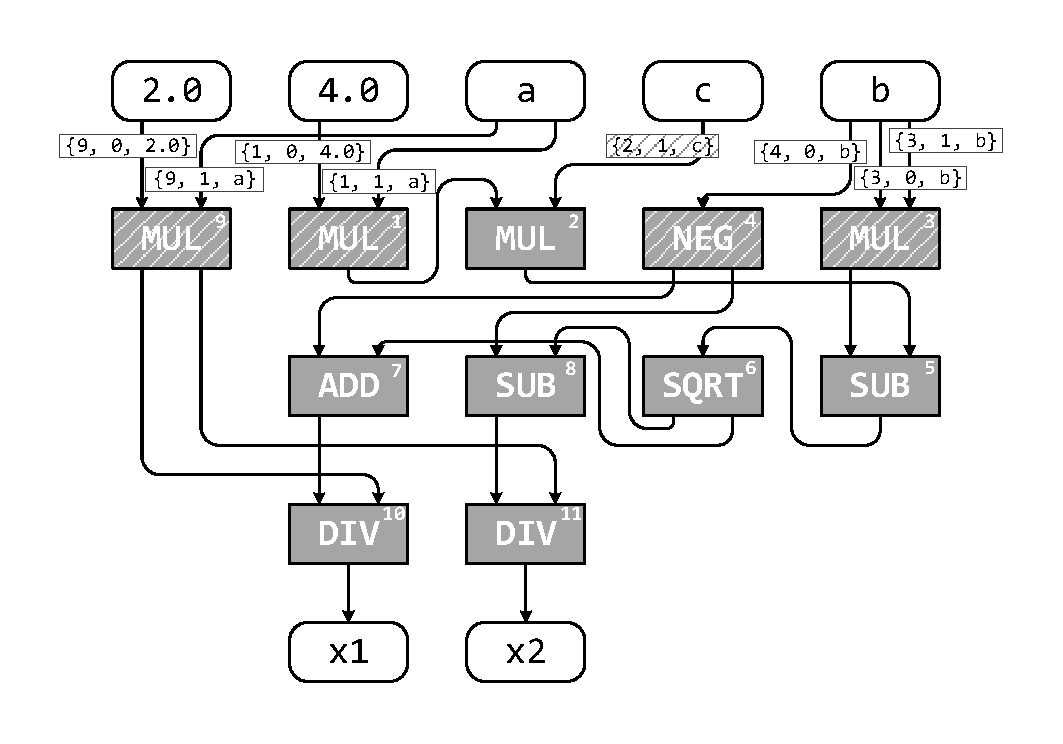
\includegraphics[width=0.80\textwidth]{pics/dataflow.pdf}
\captionstyle{normal}\caption{The dataflow graph of a linear section in the calculation of the expressions \\ of the roots of the quadratic equation.}\label{fig:dataflow}
\end{figure}

Figure~\ref{fig:dataflow} shows us dataflow graph in the initial time when none of the instructions have been completed yet.
In this figure in the arcs, we can see those tokens, which are ready and transfer at relevant instructions.
For example, for the instruction 9 MUL two tokens are ready: $\{9, 0, 2.0\}$ (9 -- number of instruction, 0 -- number of argument, 2.0 -- real number), $\{9, 1, a\}$ (9 -- number of instruction, 1 -- number of argument, $a$ -- real number).
I.e. both arguments for the instruction 9 MUL are ready and instruction can be execute.
After execution tokens, which has arguments, deletes, and at the instructions 10 DIV and 11 DIV along the output arcs will transfer tokens with the results from instruction 9 MUL.

If we will view another instruction 2 MUL we can see that it got only one ready argument (token $\{2, 1, c\}$).
First argument will be formed only after execution of instruction 1 MUL.

Thereby, all of the instructions in the presented graph will be processed while needed values will not be received in the tokens at output arcs from the instructions 10 DIV and 11 DIV.

The realization of instructions semantic in the dataflow processor emulator has no different from the same functional in the traditional processor emulator.

Central functional element for ensure operability of the dataflow processor is as named content-addressable memory.

Content-addressable token memory is a repository of tokens that are currently created and are being executed in the program.
Wherein, if it turns out that there is all needed arguments at the content-addressable memory for anyone of commands, they immediately deletes for content-addressable memory and forward for the execution in the command.
Thereby, at any given time in the content-addressable memory are only those arguments, which are still waiting missing arguments for some instructions.
I.e. at conditionally the first moment of time shows at Figure~\ref{fig:dataflow}, in the content-addressable token memory is only one token $\{2, 1, c\}$, which are still waiting its pair, whereas the commands 9 MUL, 1 MUL, 4 NEG, 3 MUL are already ready for execution and being in the command’s buffer together with the sets of their arguments.

The dataflow processors approach resolves any threads of control into separate instructions that are ready to execute as soon as all required operands available \cite{silc}. 
At the Figure~\ref{fig:dataflow} shaded the token, which is in the content-addressable memory and so the commands, which are ready to execute.

\begin{figure}[h]
\setcaptionmargin{5mm}
\onelinecaptionsfalse % if the caption is multiline
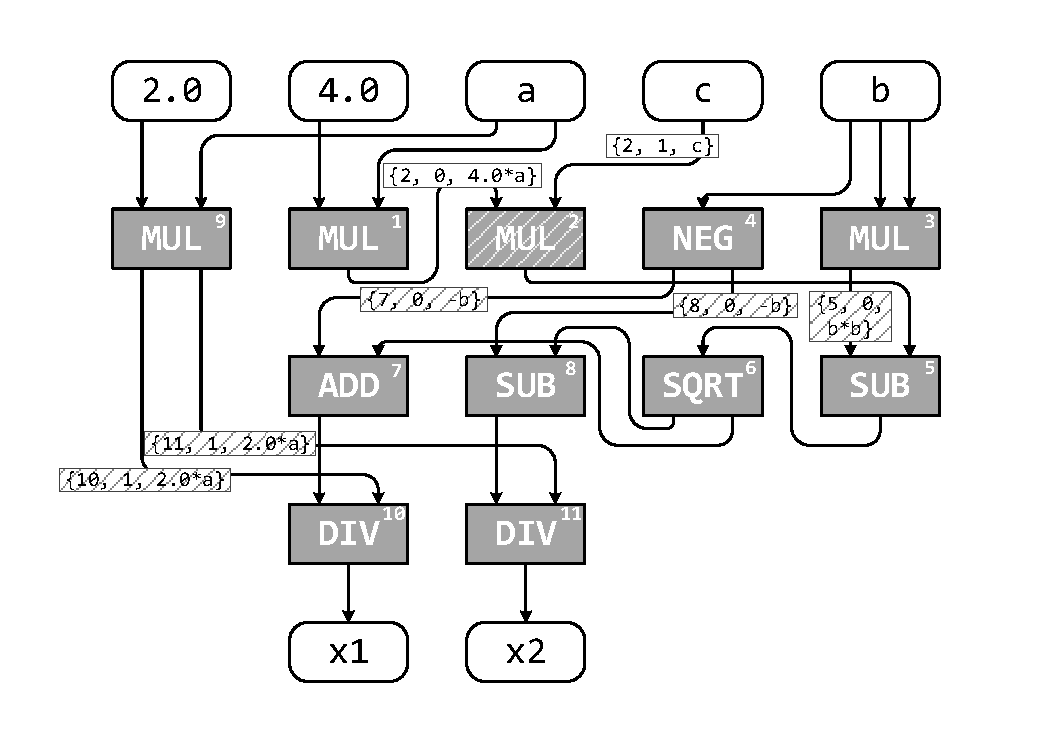
\includegraphics[width=0.80\textwidth]{pics/dataflow2.pdf}
\captionstyle{normal}\caption{The dataflow graph of the linear section when calculating the expressions of the roots of the quadratic equation before executing the 2 MUL instruction.}\label{fig:dataflow2}
\end{figure}

After the execution of the instructions 9 MUL, 1 MUL, 4 NEG and 3 MUL the only instruction is ready to execute is 2 MUL.
The machine state of this instruction before the execution shows at Figure~\ref{fig:dataflow2}.
At this Figure we can see instruction 2 MUL which are ready to execute, and also some tokens caught it the content-addressable memory.
Further execution of the program is similar and at the end, we come to the formation of two tokens on the output arcs of operations 10 DIV and 11 DIV, which will be send to their consumer instructions after that.

In the same processors, an overflow of the content-addressable memory is unacceptable, that is why the content-addressable memory must have high capacity and be fast at the same time, which is difficult to realize into practice.
That is the point to realize the emulator, which will help to get closer to creating such the dataflow processor while revealing all possible errors and shortcomings.

\section{Architecture of dataflow processor emulator}

Рассмотрим архитектуру эмулятора потокового процессора в общем виде, представленную на Figure~\ref{fig:big-scheme}.

\begin{figure}[h!]
\setcaptionmargin{5mm}
\onelinecaptionsfalse
\center{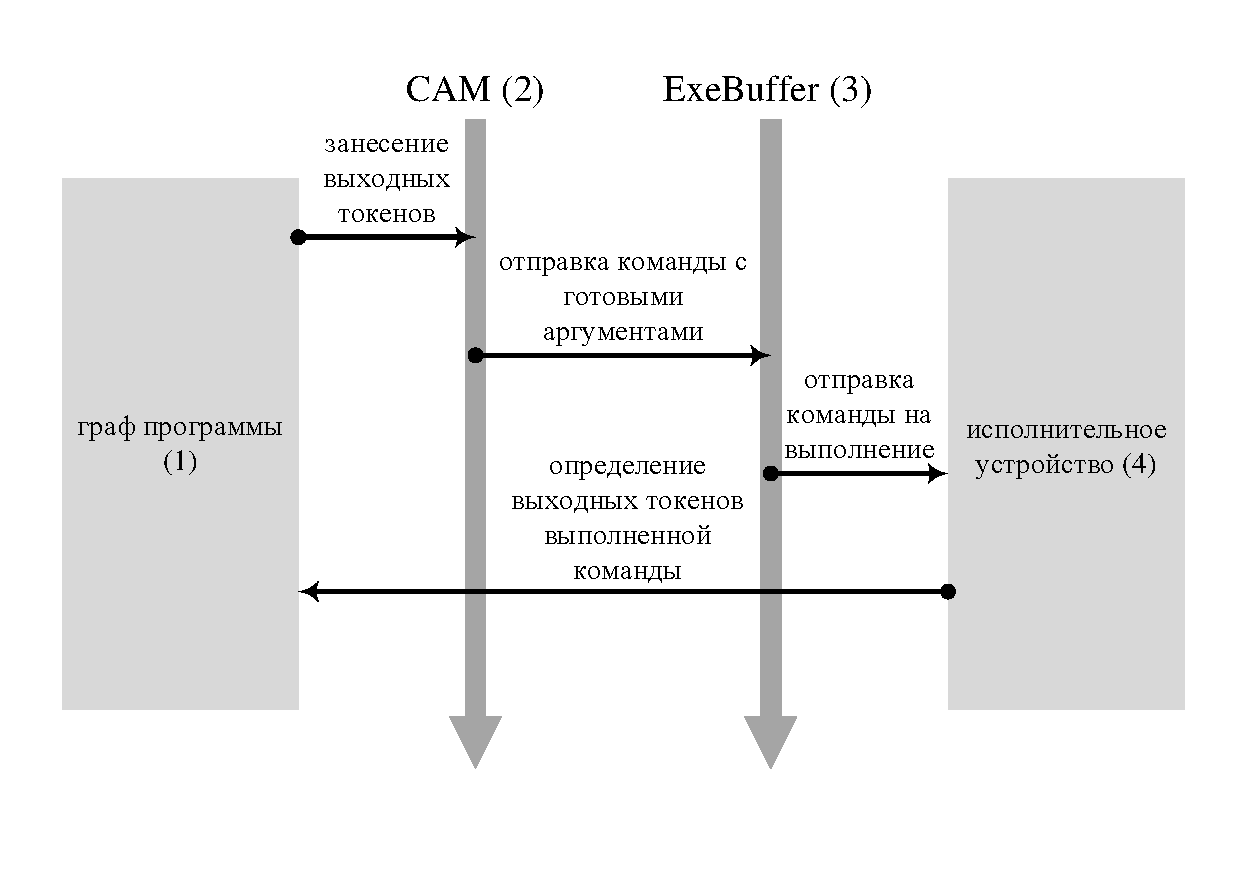
\includegraphics[width=0.80\textwidth]{pics/big-scheme.pdf}}
\captionstyle{normal}\caption{Общая схема архитектуры потокового процессора.}
\label{fig:big-scheme}
\end{figure}

Рассмотрим основные объекты, представленные на Figure~\ref{fig:big-scheme}.
Номером 1 обозначена программа, являющаяся входными данными для эмулятора, и представленная в виде ориентированного графа.
Номером 2 обозначен процесс, обслуживающий ассоциативную память токенов, которая служит для сбора аргументов отдельных команд.
Номером 3 обозначен буфер (очередь) готовых команд, которые могут быть переданы на исполнение.
Исполнительное устройство, которое в данной схеме не разделяется на скалярное и векторное, обозначено номером 4.

Между описанными объектами предусмотрены следующие варианты взаимодействия.
В первый момент времени по графу программы определяются входные токены (которые могут быть сформированы до выполнения инструкций), данные токены поступают в CAM.
Процесс, обслуживающий CAM, выполняется непрерывно.
Как только внутри CAM обнаруживается набор токенов, который является полным набором аргументов для какой-либо команды, то эта команда сразу же отправляется в буфер команд, готовых к исполнению.
Процесс, обслуживающий буфер исполнения, также выполняется непрерывно.
Единственная его задача состоит в том, чтобы оправлять команды из буфера поочередно на исполнение.
После того как на исполнительном устройстве выполнена очередная команда, происходит определение выходных токенов этой команды (с помощью графа программы), а дальше эти токены снова передаются в CAM.
Данный цикл обмена информацией между элементами эмулятора продолжается до тех пор, пока не будет выполнена команда завершения работы программы.

Таким образом, архитектура потокового процессора описана в терминах отдельных процессов, которые взаимодействуют между собой с помощью обмена сообщениями.
При этом у эмулятора отсутствует глобальное состояние, что соответствует идеологии потокового процессора.
Для реализации эмулятора потокового процессора был выбран язык программирования Erlang \cite{Armstrong,Cesarini}.
Язык программирования Erlang является функциональным языком, который предназначен для реализации отдельных параллельно выполняющихся процессов, обменивающихся сообщениями.
Обмен сообщениями между процессами является единственным способом обеспечения коммуникации между процессами (в языке отсутствует понятие разделяемой памяти), он поддержан на синтаксическом уровне.
Параллельность выполнения процессов является естественным поведением языка, поэтому не требуется реализовывать дополнительные инструменты для обеспечения взаимодействия элементов системы.

Если рассматривать элементы эмулятора потокового процессора, то отдельный интерес представляет реализация ассоциативной памяти токенов.
Реализация исполнительного устройства принципиально не отличается от реализации в эмуляторе классического процессора (реализация семантики инструкций, которые по токенам входных данных выполняют создание выходных токенов).
Буфер команд, готовых к исполнению, представляет собой просто очередь команд, поэтому его реалиация также тривиальна.
Рассмотрим реализацию ключевого элемента потокового процессора -- ассоциативную память токенов.

\begin{lstlisting}[caption={Implementation of the logic of the contest-addressable token memory.},label={lst:assoc}]
set_token({CId, E, _} = T, Args, D) when (Args > 1) ->
	FullEntries = lists:seq(0, Args - 1, 1),
	ET = {E, T},
	case dict:find(CId, D) of
		error ->
			dict:append(CId, ET, D);
		{ok, Vs} ->
			{Es, Ts} = lists:unzip(lists:sort(Vs ++ [ET])),
			case Es of
				FullEntries ->
					{Ts, dict:erase(CId, D)};
				_ ->
					dict:append(CId, ET, D)
			end
	end.
\end{lstlisting}

At Listing~\ref{lst:assoc} there is the compact logic implementation of content-addressable token memory in the Erlang programming language.
All the logics realize with one function $set\_token$ with three arguments: $T$ -- added token (which consists of the instructions identifier $CId$, number of argument $E$, and dates), $Args$ -- the number of arguments of the instruction for which the token is added, $D$ -- dictionary which token content-addressable memory is implemented.
The function logic turns to the next: to extract from the dictionary all the tokens, which are associated with the key $CId$, and check if they close all the arguments of considered instruction (i.e. numbers of the arguments form a sequence $[0, 1, .. Args - 1]$.).
If the added token is the last missing argument of the considered instruction, then we need to extract all the tokens form the dictionary and return them back in the form of list for executing the instruction (line 11).
Otherwise token should be added in the dictionary tying it to a key $CId$ (lines 6 and 13).

Note that the most simplified implementation is given.
It is not considered possibility of using the token state for instructions identify from different function calls or from different cycles iteration (for completeness as a key of dictionary together with instruction identifier $CId$ should also use the token state).
In the given implementation, exception handling also is not considered.
For example, sequential addition of two token in the content-addressable memory that are the same argument of the same instruction should cause the error.
However, despite the incompleteness of implementation, shows here logic allows providing functionality of the content-addressable token memory, which needed for execution of the dataflow processor’s program.

In the dataflow processor, communication between two instructions is much quicker if these instructions are allocated to the same processing element.
Thus a program may run much faster if its instructions are clustered to minimize communication traffic between clusters and each cluster is allocated to one processing element.
Since it will be handling significantly less packet traffic, the communication network of the dataflow processor will be simpler and less expensive than the distribution network in the cell block architecture.
Whether the cost reduction justifies the additional programming effort is a matter of debate, contingent on the area of application, the technology of fabrication, and the time frame under consideration \cite{Dennis}.

\section{Conclusion}

The article discusses the differences in the implementation of an executable program designed for a processor with von Neumann architecture and for a dataflow processor.
The differences between the use-define graph and the dataflow graph are shown, which reflect the program logic within the linear section.
The necessary element of dataflow processor’s realization shown -- content-addressable token memory with which is able to storage and quick search the ready-made tokens for the commands, which may transfer for execution.
A compact implementation of the content-addressable token memory for instructions with an arbitrary number of iterations is given.
That realization can be expanded for any program for the dataflow processor including which use cycles and function calls (including recursive).
This approach to organizing of the content-addressable token memory used in the implementation of the vector processor with dataflow architecture emulator, which is developing at the JSCC RAS.

\begin{acknowledgments}
The work has been done at the JSCC RAS as part of the state assignment for the topic 0065-2019-0016 (reg. no. AAAA-A19-119011590098-8).
The supercomputer MVS-10P, located at the JSCC RAS, was used for calculations during the research.
\end{acknowledgments}

\begin{thebibliography}{99}

\bibitem{fine-grained-prl}
\refitem{article}
N.~A.~Dikarev, B.~M.~Shabanov, A.~S.~Shmelev, {\it ``The use of fine-grained parallelism in dataflow processor"}, Problems of developing promising micro- and nanoelectronic systems (MES), {\bf 2}, pp.~144--150 (2016).

\bibitem{multithreading}
\refitem{article}
G.~V.~Papadopoulos, K.~R.~Traub, {\it ``Multithreading: a revisionist view of
dataflow architectures"}, Proc. 18-th Ann. Symp. on Computer Architecture,
ISCA ’91 (Toronto, Ontario, Canada, May 27–30, 1991), ACM, New York), pp.~342--351 (1991).

\bibitem{vpp}
\refitem{article}
N.~A.~Dikarev, B.~M.~Shabanov, {\it ``Vector dataflow processor"}, IZVESTIYA SFedU, {\bf 10}(54), pp.~80--85 (2005).

\bibitem{terada}
\refitem{article}
H.~Terada, {\it ``DDMP’s: Self-Timed Super-Pipelined Data-Driven Multimedia Processors."}, Proceedings of the IEEE, {\bf 2}(86), pp.~282--296 (1999).

\bibitem{popov}
\refitem{article}
R.~I.~Popov, {\it ``Application of stream computer models in designing specialized processors."}, Scientific and Technical Journal of Information Technologies, Mechanics and Optics, {\bf 5}(75), pp.~77--81 (2011).

\bibitem{Muchnick}
\refitem{book}
S.~S.~Muchnick, {\it ``Advanced Compiler Design \& Implementation."}, Academic Press (1997).

\bibitem{Aho}
\refitem{book}
A.~V.~Aho, M.~S.~Lam, R.~Sethi, J.~D.~Ullman, {\it ``Compilers. Principles, Techniques, \& Tools."}, Addison-Wesley (2007).

\bibitem{Wiley}
\refitem{book}
J.~Wiley, {\it ``Dataflow Computers: Their History and Future. \& Wiley Encyclopedia of Computer Science and Engineering, edited by Benjamin War"}, John Wiley and Sons, Inc (2008).

\bibitem{silc}
\refitem{book}
J.~Silc, B.~Robic, T.~Unqerer, {\it ``Processor Architecture: From Dataflow to Superscalar and Beyond"}, Springer Science and Business Media, (2012).

\bibitem{Armstrong}
\refitem{book}
J.~Armstrong, {\it ``Programming Erlang. Software for a Concurrent World."}, Pragmatic Programmers (2013).

\bibitem{Cesarini}
\refitem{book}
F.~Cesarini, S.~Thompson, {\it ``Erlang programming."}, O'Reilly (2009).

\bibitem{Dennis}
\refitem{article}
J.~B.~Dennis, {\it ``Data Flow Supercomputers."}, MIT Laboratory for Computer Science, {\bf 13}, pp.~48--56 (1980).

\end{thebibliography}

\end{document}
